\documentclass[10pt,a4paper]{article}
\usepackage[top=14mm,bottom=15mm,left=16mm,right=16mm,headheight=12pt,headsep=5mm,footskip=8mm]{geometry}
\usepackage[T1]{fontenc}
\usepackage{lmodern,microtype}
\usepackage{array,tabularx,booktabs,xcolor}
\usepackage{tikz}
\usetikzlibrary{arrows.meta,positioning,fit,backgrounds}
\usepackage{enumitem,fancyhdr}
\usepackage[hidelinks]{hyperref}
\definecolor{forest}{HTML}{185547}
\definecolor{ink}{HTML}{263530}
\definecolor{muted}{HTML}{596760}
\definecolor{tint}{HTML}{EDF4F1}
\definecolor{line}{HTML}{A7BFB4}
\hypersetup{pdftitle={ReCycleGuard - Review 2 System Design},pdfauthor={R V Abhishek; H Sampreeth Bhat; Sushanth S; Vedantha Vinay Vernekar}}
\setlength{\parindent}{0pt}
\setlength{\parskip}{3pt}
\setlength{\tabcolsep}{4pt}
\renewcommand{\arraystretch}{1.10}
\newcolumntype{Y}{>{\raggedright\arraybackslash}X}
\newcolumntype{L}[1]{>{\raggedright\arraybackslash}p{#1}}
\newcommand{\sect}[1]{\par\vspace{5pt}{\sffamily\bfseries\color{forest}\large #1}\par\vspace{2pt}}
\newcommand{\sub}[1]{\par\vspace{3pt}{\sffamily\bfseries\color{forest}#1}\par}
\newcommand{\pagehead}[2]{{\sffamily\fontsize{8}{10}\selectfont\bfseries\color{muted}REVIEW 2\quad /\quad SYSTEM DESIGN\hfill 22 OCTOBER 2026}\par\vspace{3pt}{\sffamily\fontsize{21}{24}\selectfont\bfseries\color{forest}#1}\par{\sffamily\small\color{muted}#2}\par\vspace{3pt}{\color{forest}\hrule height .8pt}\vspace{3pt}}
\newcommand{\callout}[1]{\par\begingroup\setlength{\fboxsep}{7pt}\colorbox{tint}{\parbox{\dimexpr\linewidth-14pt}{#1}}\endgroup\par}
\newcommand{\code}[1]{\texttt{\small #1}}
\newcommand{\refitem}[3]{\par\hangindent=5mm\hangafter=1{\bfseries[#1]} #2. \href{#3}{\textcolor{forest}{Primary source}}.}
\pagestyle{fancy}\fancyhf{}
\fancyfoot[L]{\sffamily\fontsize{8}{10}\selectfont\color{muted}ReCycleGuard\quad |\quad Proposed design v1.1\quad |\quad No measured results}
\fancyfoot[R]{\sffamily\small\color{forest}\thepage\ /\ 5}
\renewcommand{\headrulewidth}{0pt}\renewcommand{\footrulewidth}{.3pt}
\tikzset{box/.style={draw=line,rounded corners=2pt,fill=tint,align=center,font=\sffamily\fontsize{8.5}{10.5}\selectfont,inner sep=5pt},arr/.style={-{Stealth[length=1.6mm]},draw=forest,line width=.6pt}}
\begin{document}\color{ink}
\pagehead{ReCycleGuard}{Agentic AI for E-Waste EPR Compliance Reconciliation}
{\sffamily\fontsize{8.5}{10.5}\selectfont Agentic AI (26CD7PEAAI) $\cdot$ B.E. CSE (Data Science), VII Semester, BMSCE\\Instructor: Dr. Kalyan Nagaraj\hfill Review: 24 October 2026}
{\small
\begin{tabularx}{\linewidth}{@{}YY@{}}
R V Abhishek (Lead) --- 1BM23CD047 & H Sampreeth Bhat --- 1BM23CD020\\
Sushanth S --- 1BM23CD063 & Vedantha Vinay Vernekar --- 1BM23CD069
\end{tabularx}}\par
\sect{1\quad Decision, scope and architecture}
\callout{\textbf{Decision supported.} Which discrepancy should the compliance officer investigate next, and what verification or correction does the evidence support? The output is a traceable working paper with calculations, citations, uncertainty and named next-action owners.}
\textbf{V1 boundary.} One synthetic producer; closed FY 2024--25; up to two specific reviewed EEE codes; supplied Au/Cu/Al/Fe obligation buckets and separately dated historical liabilities. Gold is a fixed supplied bucket; gold-specific adjustments are unsupported. V1 does not derive statutory targets from sales. A bounded single investigator operates within a human-reviewed workflow.

\textbf{Excluded.} Live portal filing, certificate trading, OTP interaction, autonomous legal certification and compensation calculation. Components, dossiers and experiments below are \emph{planned}; the repository currently contains specifications, not an implemented application.

\sub{Local application and offline evaluation boundary}
\begin{center}
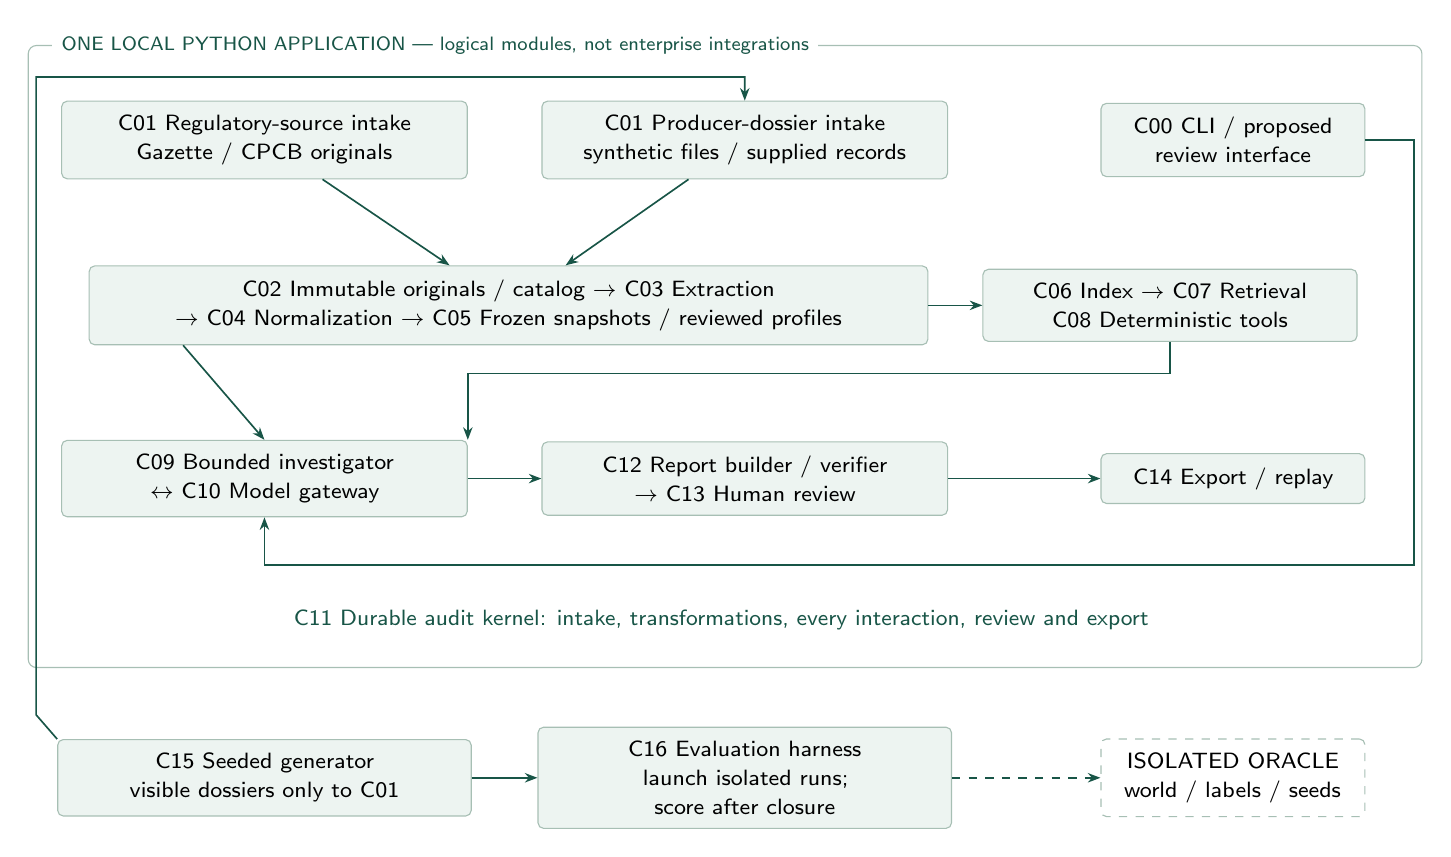
\begin{tikzpicture}[x=1mm,y=1mm]
\draw[draw=line,rounded corners=3pt] (0,0) rectangle (177,79);
\node[font=\sffamily\scriptsize,color=forest,anchor=west,fill=white] at (3,79) {ONE LOCAL PYTHON APPLICATION --- logical modules, not enterprise integrations};
\node[box,text width=48mm] (reg) at (30,67) {C01 Regulatory-source intake\\Gazette / CPCB originals};
\node[box,text width=48mm] (case) at (91,67) {C01 Producer-dossier intake\\synthetic files / supplied records};
\node[box,text width=30mm] (ui) at (153,67) {C00 CLI / proposed\\review interface};
\node[box,text width=103mm] (data) at (61,46) {C02 Immutable originals / catalog $\to$ C03 Extraction\\$\to$ C04 Normalization $\to$ C05 Frozen snapshots / reviewed profiles};
\node[box,text width=44mm] (rt) at (145,46) {C06 Index $\to$ C07 Retrieval\\C08 Deterministic tools};
\node[box,text width=48mm] (agent) at (30,24) {C09 Bounded investigator\\$\leftrightarrow$ C10 Model gateway};
\node[box,text width=48mm] (review) at (91,24) {C12 Report builder / verifier\\$\to$ C13 Human review};
\node[box,text width=30mm] (export) at (153,24) {C14 Export / replay};
\node[font=\sffamily\fontsize{8.5}{10}\selectfont,color=forest] at (88,6) {C11 Durable audit kernel: intake, transformations, every interaction, review and export};
\draw[arr] (reg)--(data);\draw[arr] (case)--(data);\draw[arr] (data)--(rt);
\draw[arr] (ui.east)--(176,67)--(176,13)--(30,13)--(agent.south);
\draw[arr] (data.south west)++(12,0)--(agent.north);
\draw[arr] (rt.south)--++(0,-4)-|(agent.north east);
\draw[arr] (agent)--(review);\draw[arr] (review)--(export);
\node[box,text width=49mm] (gen) at (30,-14) {C15 Seeded generator\\visible dossiers only to C01};
\node[box,text width=49mm] (eval) at (91,-14) {C16 Evaluation harness\\launch isolated runs; score after closure};
\node[box,fill=white,dashed,text width=30mm] (oracle) at (153,-14) {ISOLATED ORACLE\\world / labels / seeds};
\draw[arr] (gen.north west)--(1,-6)--(1,75)--(91,75)--(case.north);
\draw[arr] (gen)--(eval);\draw[arr,dashed] (eval)--(oracle);
\end{tikzpicture}
\end{center}
\vspace{-5pt}
{\small\textbf{Diagram key.} C00--C14 form the runtime; C15--C16 are offline benchmark modules. The generator produces visible evidence and separate truth. Only the evaluator can read truth after investigator artifacts close. There is no oracle path into retrieval, prompts or the review UI. C11 spans every component; arrows abbreviate control and data flow.}

\textbf{Feasibility.} Proposed stack: Python 3.11+, uv, Typer, Pydantic v2, SQLite/\code{Decimal}, PDF extraction and LangGraph checkpoints. FTS5 is the lexical baseline [5]; dense retrieval is an experiment. One local process and a single database writer keep the initial deployment manageable. Full versioned interfaces remain in \code{CONTRACTS.md} v1.1.

\newpage
\pagehead{Agent, reasoning and patterns}{2\quad Adaptive investigation with deterministic calculations}
\textbf{Agentic responsibility.} Code establishes provisional facts and arithmetic. The investigator chooses the next unresolved hypothesis, evidence inspection or rule query in response to observations. It cannot change canonical quantities. Each action stores a concise plan, expected evidence and stopping criteria; each result stores an assessment and linked plan revision. These are visible decision records, not private chain-of-thought.

\begin{center}
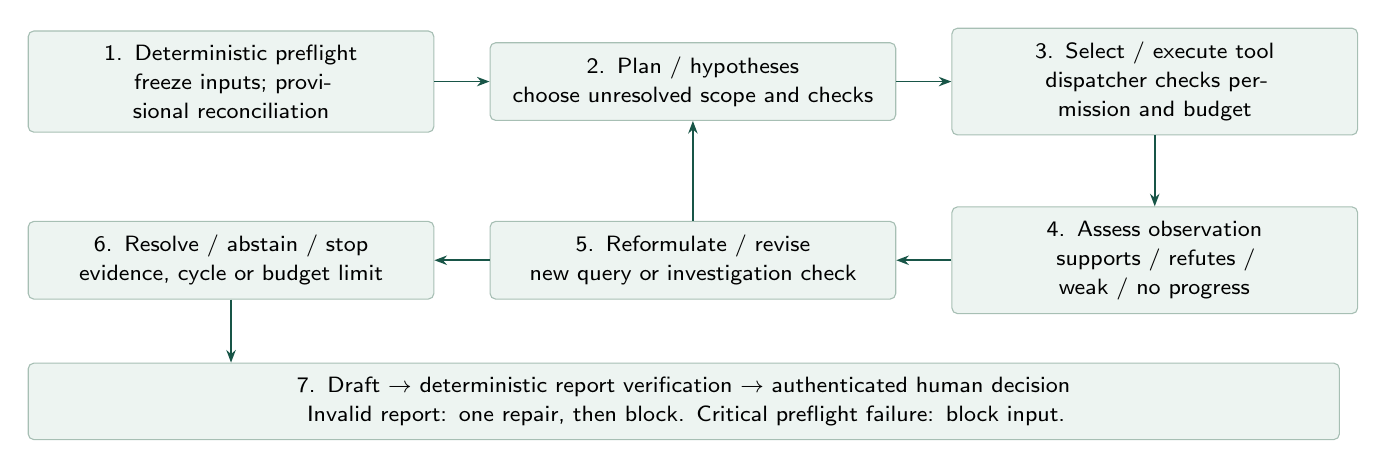
\begin{tikzpicture}[node distance=5mm and 7mm]
\node[box,text width=48mm] (pre) {1. Deterministic preflight\\freeze inputs; provisional reconciliation};
\node[box,text width=48mm,right=of pre] (plan) {2. Plan / hypotheses\\choose unresolved scope and checks};
\node[box,text width=48mm,right=of plan] (tool) {3. Select / execute tool\\dispatcher checks permission and budget};
\node[box,text width=48mm,below=9mm of tool] (obs) {4. Assess observation\\supports / refutes / weak / no progress};
\node[box,text width=48mm,left=of obs] (rev) {5. Reformulate / revise\\new query or investigation check};
\node[box,text width=48mm,left=of rev] (stop) {6. Resolve / abstain / stop\\evidence, cycle or budget limit};
\node[box,text width=163mm,below=8mm of stop.south west,anchor=north west] (report) {7. Draft $\to$ deterministic report verification $\to$ authenticated human decision\\Invalid report: one repair, then block. Critical preflight failure: block input.};
\draw[arr] (pre)--(plan);\draw[arr] (plan)--(tool);\draw[arr] (tool)--(obs);
\draw[arr] (obs)--(rev);\draw[arr] (rev)--(stop);\draw[arr] (rev.north)--(plan.south);
\draw[arr] (stop.south)--(report.north -| stop.south);
\end{tikzpicture}
\end{center}
\vspace{-5pt}
\sub{Selected patterns and why they fit}
{\small
\begin{tabularx}{\linewidth}{@{}L{29mm}Y@{}}\toprule
\textbf{Pattern} & \textbf{ReCycleGuard choice and justification}\\\midrule
Tool use & Exact joins, units, quantities, lifecycle checks and allocation conservation remain deterministic C08 operations.\\
Agentic RAG & C09 chooses queries, assesses evidence grades and re-queries weak results through C07; retrieval is a decision, not a fixed prompt attachment.\\
Planning / reflection & Persist plans, observations, mistakes and revisions with predecessor links; assess whether the next check adds evidence.\\
Human review & C13 binds approval, rejection, changes and escalation to exact report and input versions; the agent cannot authenticate a reviewer.\\
Multi-agent & Optional collector/auditor experiment using the same dispatcher and authorized evidence. It is not a prerequisite for v1.\\
Durable workflow & LangGraph checkpoints support recovery [6]. Committed application operations and the C11 audit ledger remain authoritative.\\\bottomrule
\end{tabularx}}\par
\sub{Worked adaptation: pending payment is not supported fulfillment}
\callout{\textbf{Initial observation:} a 100 kg synthetic target has one supported 55 kg allocation, observed twice, and a paid 25 kg item with pending transfer/allocation. Supported fulfillment stays \textbf{55 kg}; apparent gap is \textbf{45 kg}; \textbf{25 kg remains pending}. The two observations do not create 110 kg.}
The investigator tests whether the pending item has a completed, eligible allocation. Payment or a newer account snapshot alone does not resolve the finding. Only a later evidenced and reviewed \textbf{25 kg allocation} supports a new version with \textbf{80 kg} fulfillment and a \textbf{20 kg} apparent gap. Without that support, abstain on the unresolved allocation and name the required evidence. A changed dossier starts a new authorized run linked to its parent.

\sub{Configurable model gateway and bounded execution}
C10 is the sole provider boundary. Select a configuration only after checking structured/schema-constrained responses, typed tool proposals, sufficient context, usage/timing capture and reliability on representative tasks. Pin model/provider, prompt, tool schema and response schema per run. No model is selected here; no automatic fallback is assumed. Optional embeddings use the same gateway and frozen manifests.

Validate every proposal before dispatch. Retain exact permitted requests, responses and errors; secrets stay outside the archive. Permit one budgeted retry per retryable attempt, including invalid structured output if policy allows. Unrecoverable provider failure ends the run; unknown external completion is recorded as \code{OUTCOME\_UNKNOWN}. Resume uses committed operations and consumed budgets, not a fresh allowance. Runtime ceilings are configuration, not measured performance.

\newpage
\pagehead{Knowledge, memory and storage}{3\quad Preserve originals; retrieve only eligible, versioned evidence}
\sub{Sources and structure-aware extraction}
The planned normative corpus uses official Gazette instruments and CPCB framework/SOP/FAQ/instructions. The 2022 Rules, G.S.R. 801(E), commence on 1 April 2023 [1]; the 8 March 2024 amendment includes Rule 9A [2]. Retain base text and amendments as separate versions rather than declaring one PDF a consolidated rulebook. Clause-specific applicability must be reviewed; a source-class ranking alone cannot decide a legal conflict.

For each source, preserve original bytes, URL, acquisition/capture time, source class, exact instrument/version, commencement, applicable interval, provision path, page/table/cell locator and rights-review decision. Gazette rules, orders, frameworks, SOPs, instructions, FAQs and notice leads remain distinct classes. Public hosting does not automatically authorize model use or redistribution; unknown rights remain \code{REVIEW\_REQUIRED}.

Structure-aware extraction preserves clauses, headings, table rows, headers and footnotes. Every submitted file gets a receipt; every discovered page/row gets a parsed, quarantined, excluded or unavailable disposition. Preserve raw OCR values and validation issues; critical identifiers need deterministic validation or human confirmation. A corrupt file or missing page is not zero business activity.

\textbf{Data roles.} Public aggregate statistics provide context only, never producer transaction evidence. Original synthetic dossiers are the proposed evaluation evidence: manifests, obligations, certificate events, allocations, account snapshots, commercial records and optional PDF/CSV renderings. JSONL records must resolve to declared original evidence; there is no clean answer table secretly available to the investigator.

\sub{Retrieval and evidence grading}
C06 builds a frozen SQLite FTS5 lexical/BM25 index [5]. C07 filters by access, regime, role and reviewed temporal applicability, including eligible general provisions. Optional dense retrieval is adopted only if measured gains justify it; it uses the same eligibility and provenance contract. No embedding model or vector service is selected.

Expand parent headers, footnotes and applicable amendment counterparts under a recorded traversal policy (default depth 2, at most 20 nodes). Grade \textbf{authority, temporal applicability, direct support, completeness and contradiction} separately. Missing signed authority is a lead, not a definitive rule citation. Ambiguous locators or conflicting applicability require abstention/escalation. Preserve ranked candidates, expansion edges, grading, query revisions, not-scored items and context exclusions against full snapshot membership.

\sub{Storage and memory: separate meanings, explicit lineage}
{\small
\begin{tabularx}{\linewidth}{@{}L{37mm}Y L{34mm}@{}}\toprule
\textbf{Layer} & \textbf{Contents and authoritative meaning} & \textbf{Planned storage}\\\midrule
Original files & Immutable exact PDF/CSV/JSON/HTML bytes, receipt, hash, rights and access scope. & Content-addressed objects + catalog\\
Extracted observations & What a specific source page/row says; raw values, revisions and coverage. & JSONL/page text + SQLite links\\
Events and credit lots & Distinct lifecycle events; supported equivalence links; underlying eligible capacity. & SQLite typed entities / assertions\\
Supported allocations & Evidenced use of a credit lot against one dated liability bucket; active revisions only. & SQLite allocation ledger\\
Account comparisons & Captured reported balance, compared with ledger; never an invented allocation. & SQLite observations / deltas\\
Snapshots and audit & Frozen case/corpus/profile/index membership, full operation payloads, reports and reviews. & Canonical manifests, blobs, runtime SQLite\\
Hidden benchmark truth & World ledger, corruptions, labels, seeds and visible-evidence expectations; no runtime table. & Separate evaluator-only root\\\bottomrule
\end{tabularx}}\par
\sub{Working memory versus persistent case history}
C09 run state and LangGraph checkpoints hold the finding queue, plans, observations, current status and budgets. SQLite plus immutable artifacts retain case history, findings and human decisions. Previous interpretations may aid navigation but are \emph{never automatically reused as legal truth}; each run pins its own reviewed profile and source versions.

\callout{\textbf{Retention is broader than model context.} Originals and observations remain available under their access policy even when never retrieved, cited or sent to the model. Checkpoints and indexes are derived; they do not replace evidence or the authoritative audit ledger.}

\newpage
\pagehead{Tools, contracts and governance}{4\quad Typed execution boundaries and accountable human decisions}
\textbf{Shared protocol.} Contracts v1.1 pin case/corpus/profile/index and code/prompt/policy versions. Each operation carries actor capability, operation/attempt IDs, idempotency key and audit refs. \code{ServiceResult<T>} returns status, complete result blob, issues and typed provenance/locator dependencies. Decimal quantities are strings, not binary floats. C07/C08 examples follow; full contracts: \code{docs/design/CONTRACTS.md}, §§2, 6--7.

{\fontsize{9}{11}\selectfont
\begin{tabularx}{\linewidth}{@{}L{38mm}Y Y@{}}\toprule
\textbf{Tool / owner} & \textbf{Version-bound input} & \textbf{Structured output / explicit failure}\\\midrule
\code{inspect\_evidence} (C08) & Artifact, observation or record refs within permitted scope. & Raw/parsed values, provenance, issues; \code{ACCESS\_DENIED}, \code{MISSING\_ARTIFACT}.\\
\code{resolve\_locator} (C07) & Corpus, source alias/version, legal path, question basis, applicability, expansion policy. & Exact provision revision + evidence bundle; \code{APPLICABILITY\_UNRESOLVED}.\\
\code{trace\_certificate} (C08) & Certificate/event refs in the pinned case. & Observations, equivalence, event/lot and allocation history; ambiguity stays explicit.\\
\code{compute\_reconciliation} (C08) & Case/profile, bucket IDs and expected input-membership digest. & Required/supported/pending, gaps and provenance; dimension, precision or profile errors.\\
\code{compare\_return\_draft} (C08) & Draft revision, calculation IDs, section dispositions, deadline refs. & Bucket deltas + scoped readiness; missing/unsupported sections; undetermined applicability.\\\bottomrule
\end{tabularx}}\par
\vspace{2pt}
C08 includes historical allocations and conflicts from the frozen snapshot; model-selected subsets cannot hide liabilities. Unknown/partial data and tool failure remain explicit.

\sub{Evidence capabilities and deterministic safeguards}
\textbf{Different documents establish different facts.} Payment supports a commercial fact; weight tickets support physical movement; a portal snapshot reports an account position. None alone establishes eligible liability allocation. Recycler EEE capability and compatible metal are separate checks [3,4].

For each metal/liability bucket, required = supplied target + approved signed adjustments; supported = active, evidenced allocations; signed gap = required $-$ supported. Preserve shortfall, surplus and pending separately. Never add metal gaps into a legally meaningful total. Account delta = portal reported $-$ ledger supported; missing portal evidence is null, not zero.

\textbf{Conservation and identity.} Total active use across all events and prior/current buckets cannot exceed supported credit-lot capacity. F02 repeated observations require an authoritative event ID or a complete compound key plus source continuity excluding indistinguishable events; overlap alone is insufficient. F03 legitimate stages sharing a certificate remain distinct events. Check F09 expiry/cancellation. Assess earlier-liability priority \emph{at allocation time}; unknown ordering remains unresolved. Achievement, credit-event and filing cut-offs are separate, source-backed deadline entries [1,2].

\sub{Permissions, stopping and report verification}
Model-accessible tools read/check and write new derivations, findings or report drafts. Trusted review handlers alone approve profiles/decisions and link supplied acknowledgments. The model cannot mutate source records or portal state, execute arbitrary SQL, shell or dynamic code. Evidence is untrusted input: hostile text is preserved but cannot change tool capabilities, profiles or review status. Redact model inputs through access policy and retain linked permitted originals.

Default limits: \textbf{8 investigative tool actions per finding, 2 query reformulations, 1 report repair and 1 retry per retryable attempt}; case-wide action/token/cost/wall-time limits are required configuration. Bound preflight/verification separately. Missing evidence, rule conflicts, no progress or budget exhaustion produce scoped abstention; critical input failure blocks input, invalid unrepaired output blocks output, and unrecoverable provider/audit failure stops execution. C12 rejects legal-compliance verdicts, intent/fraud/concealment allegations and compensation amounts; qualification cannot bypass the prohibition.

\sub{Version-bound review and complete audit lineage}
\textbf{Originals $\to$ observations $\to$ calculations $\to$ findings $\to$ report $\to$ review.} C11 retains full tool/model inputs, outputs/errors, contexts, omissions, timing and turn links. Commit domain changes and audit together; audit failure blocks progress. Hash chains detect changes relative to retained anchors.

APPROVE moves \code{AWAITING\_REVIEW} to \code{COMPLETED}; REJECT or REQUEST\_CHANGES to \code{BLOCKED\_OUTPUT}; ESCALATE remains awaiting an external decision. Bind decisions to exact report/dependency hashes. Corrections create a new authorized parent-linked run; approval never transfers. Explicit manual closure records \code{CLOSED\_WITHOUT\_DECISION}, never approval. Approved report does not mean filed return.

\newpage
\pagehead{Evaluation and feasibility}{5\quad Proposed assessment, ownership, limitations and references}
\sub{Benchmark and controlled comparisons}
Plan \textbf{48 synthetic dossiers: 24 development and 24 held-out}, split by entity/template/fault combination rather than random rows. Cover all shared families: F01 clean; F02 overlapping export; F03 multistage ID reuse; F04 unit/dimension mix; F05 entity alias; F06 stale snapshot; F07 paid/no transfer; F08 prior arrears; F09 expired/cancelled; F10 capability mismatch; F11 wrong-period rule; F12 unseen notice; F13 weight basis; F14 unsupported regime; F15 extraction loss; F16 injection. This is a pilot target, not an existing or validated dataset.

C15 generates world facts, renders visible evidence and injects faults. Independent reviewed fixtures/calculations establish reference answers; the production calculator is not its own sole oracle. Distinguish hidden world truth from conclusions justified by visible evidence. Investigators get no truth mount, labels, seeds or answer-bearing filenames; C16 scores closed run artifacts, with evaluator views separate from review UI. Test and audit attempted oracle access.

Compare on identical visible inputs and frozen profiles: \textbf{(A)} deterministic reconciliation; \textbf{(B)} fixed retrieval plus tools; \textbf{(C)} bounded single investigator; \textbf{(D)} optional collector/auditor. Record actual evidence/call budgets, all failures and repeated trials; freeze configuration before held-out scoring.

{\fontsize{9}{11}\selectfont
\begin{tabularx}{\linewidth}{@{}L{41mm}Y@{}}\toprule
\textbf{Metric} & \textbf{Definition and interpretation}\\\midrule
Exact balance agreement & Fraction of eligible buckets exactly matching independent decimal references; report every mismatch, pending amount and comparison delta.\\
Discrepancy precision / recall & Correct discrepancy findings / all predicted; detected reference discrepancies / all reference discrepancies. F01 tests false positives.\\
Resolution / abstention & Evidence-supported resolutions and correct abstentions over corresponding oracle scopes; do not reward guessing hidden truth.\\
Citation / temporal correctness & Claim citations that directly support the claim and apply to its role, regime and date / citations assessed, using reviewed references.\\
Unsupported / prohibited rates & Unsupported claims / assessed claims; prohibited generated verdicts / assessed verdict candidates. Record forbidden tool attempts separately.\\
Steps, latency and cost & Mean investigative actions per task; measured latency p50/p95 and failures; provider cost per task (unknown cost stays null).\\
Repeated-run reliability & Fraction of repeated trials meeting correctness/safety gates; report outcome variation with trial counts and configuration.\\
Evidence / audit coverage & Received assets and discovered pages/rows with terminal accounting; operations/turns with complete payloads and lineage / expected totals.\\\bottomrule
\end{tabularx}}\par
\textbf{Hard acceptance gates.} Exact supported arithmetic against independent references; complete evidence accounting and operation audit coverage; \textbf{zero prohibited generated verdicts in released reports}. Block or qualify unsupported scopes, never invent certainty. Report raw counts alongside rates; unknown coverage is not 100\%. Accuracy, latency, cost and collaboration gains remain \emph{unmeasured}. Limits are configured budgets, not benchmark achievements.

\sub{Implementation order and proposed ownership}
Freeze contracts/audit first $\to$ ingestion/snapshots and generator $\to$ deterministic baseline $\to$ lexical retrieval $\to$ bounded agent $\to$ review/export/evaluation. Abhishek: integration/contracts, C00/C09/C10; Sampreeth: sources/applicability, C01/C05--C07; Sushanth: normalization/calculation and reference fixtures, C03/C04/C08/C15; Vedantha: evidence/audit presentation, review/export/evaluation integration, C02/C11--C14/C16. Shared boundaries are reviewed by all; reference calculations require independent cross-review. Ownership is proposed, not an external commitment.

\textbf{Key limits.} Synthetic-only pilot cannot establish production accuracy or legal validity. Source rights, exact EEE codes and reviewed profiles remain activation decisions. Provider/context limits, OCR and dense retrieval require measured selection. Numerical/citation checks cannot prove semantic legal correctness. Local hashes need retained anchors; private evidence requires separate publication/redaction review.

\sub{Primary references and specification authority}
{\fontsize{8}{9.5}\selectfont\setlength{\parskip}{2pt}
\refitem{1}{MoEFCC. E-Waste (Management) Rules, 2022, G.S.R. 801(E), 2 Nov 2022; Rules 6, 14--15 and Schedules III--IV}{https://eprewaste.cpcb.gov.in/assets/PDF/e-waste_rules_2022.pdf}
\refitem{2}{MoEFCC. Amendment Rules, 2024, G.S.R. 164(E), 8 Mar 2024; inserted Rule 9A}{https://eprewaste.cpcb.gov.in/assets/PDF/Amendment-Rules-2024.pdf}
\refitem{3}{CPCB. Framework for generation of EPR Certificate; main provisions and Annexure I}{https://eprewaste.cpcb.gov.in/assets/PDF/Framework.pdf}
\refitem{4}{CPCB. FAQ under E-Waste Rules, 23 Jan 2024, Section C}{https://eprewaste.cpcb.gov.in/assets/PDF/faqewaste.pdf}
\refitem{5}{SQLite. FTS5 Extension, lexical indexing and BM25}{https://www.sqlite.org/fts5.html}
\refitem{6}{LangChain. LangGraph persistence and checkpoints}{https://docs.langchain.com/oss/python/langgraph/persistence}
\par\textbf{Internal authority:} \code{docs/design/SYSTEM\_DESIGN.md} and \code{CONTRACTS.md}, corrected v1.1, 22 Oct 2026. This submission condenses those specifications; it does not activate a rule profile or claim a complete current legal corpus.
}
\end{document}
